\documentclass[letterpaper]{report}
\usepackage[utf8]{inputenc}
\usepackage[spanish]{babel}
\usepackage{cite,url,graphicx}
\usepackage{fullpage}
\usepackage{authblk}

%\renewcommand{\baselinestretch}{1.5}

\title{Propuesta de Tesis: \\ Calendarización de flujos de trabajo en cómputo en la nube}
\author{Fernando Aguilar Reyes}

\affil{Maestría en Ciencias en Computación \\
       Instituto Tecnológico Autónomo de México \\
     Río Hondo \#1, Progreso Tizapán, Del. Álvaro Obregón, 01080 \\
	   México, Distrito Federal \\}

\begin{document}

\maketitle

\abstract{
Los flujos de trabajo, o conjunto de tareas de un proceso, son utilizados en aplicaciones como el etiquetado de proteínas o el ajuste de cuentas bancarias al final del día. Como requieren vastos recursos computacionales, se han empleado enfoques de cómputo distribuido (clusters y grids) para ejecutar estos flujos. Sin embargo, el enfoque de cómputo en la nube ha tomado un gran interés tanto por la academia como por la industria, porque el esquema de pagos ``pay as you go'' y la elasticidad de los recursos de la nube posibilitan la ejecución de estos flujos sin necesidad de contar con infraestructura especial. Una parte importante para la ejecución de los flujos es la calendarización de sus tareas. Con ello, podríamos hacer planeaciones que maximicen el uso del sistema distribuido o que minimicen el tiempo de ejecución total. En esta propuesta de tesis, proponemos crear un calendarizador de flujos de trabajo que tome en cuenta las características únicas del enfoque de cómputo en la nube para que se pueda minimizar el tiempo de ejecución y, también, el dinero utilizado por la renta de los servicios en la nube.
}

\chapter*{Propuesta de Tesis}

\section*{Análisis de antecedentes: Revisión inicial de literatura}

\subsection*{Flujos de trabajo}

%la anotación de proteínas, el cual consiste en identificar ciertas partes de la proteína y poner una etiqueta que describa la función de dicho componente

\begin{figure}
    \begin{center}
        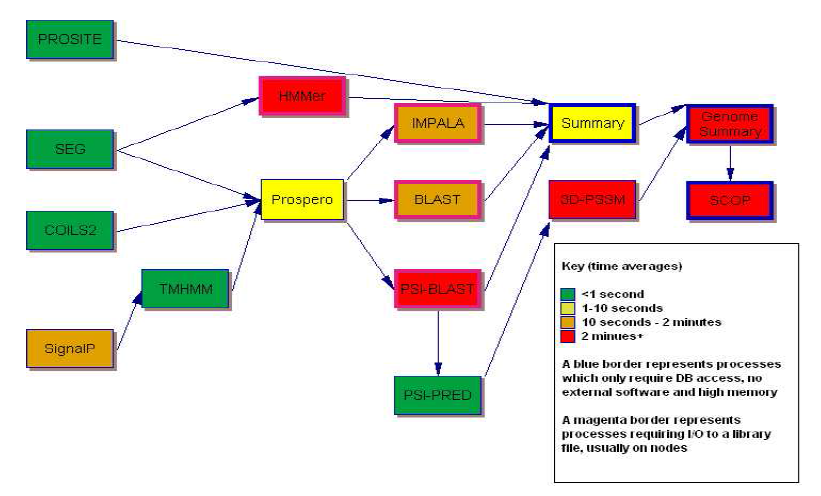
\includegraphics[width=0.8\textwidth]{imagenes/iceni-workflow}
    \end{center}
    \caption{Flujo de trabajo para la anotación de proteínas, diseñado en la Escuela Imperial de Londres para el proyecto \emph{e-Protein}}
    \label{fig:iceni-workflow}
\end{figure}

Entendemos que un flujo de trabajo, o \emph{workflow} en inglés, es un conjunto de pasos que modelan la ejecución de un proceso \cite{gutierrez2012agent}. Un ejemplo de un flujo de trabajo es el que el se desarrolló en la Escuela Imperial de Londres para el proyecto \emph{e-Protein} \cite{o2004mapping}, cuyo objetivo era la idenficación y anotación de partes de proteínas que expliquen la estructura y la función de dicha proteína.

Una proteína está compuesta de varios aminoácidos y se estima que existen al menos 500 aminoácidos diferentes \cite{wagner1983new}, dando lugar a un número muy grande de posibles proteínas. De este modo, los investigadores de la Escuela Imperial diseñaron un flujo de trabajo compuesto de varios programas especializados para hacer la anotación de proteínas. En la figura \ref{fig:iceni-workflow} podemos ver el flujo de trabajo \cite{o2004mapping}, donde las flechas indican el flujo de datos y los colores indican el tiempo de ejecución aproximado. Las cajas (o nodos) del diagrama son los diferentes programas que se utilizan para hacer el proceso de anotación de proteínas. Así, podríamos pensar que un flujo de trabajo puede ser representado por un grafo dirigido acíclico.

Por lo general, los flujos de trabajo tienen una complejidad computacional que hace prohibitiva su ejecucion en una sola computadora. Por ello, diversos enfoques se han aplicado para distribuir la ejecución de un flujo de trabajo entre varias computadoras.  De acuerdo a Buyya et al., los enfoques de cómputo más importantes para los flujos de trabajo son los \emph{clusters}, los \emph{grids} y las \emph{nubes} \cite{buyya2009cloud}. A continuación, explicaremos cada uno de los enfoques.

\begin{itemize}
\item Los \emph{clusters} son sistemas distribuidos, paralelos, compuestos de varias computadoras que son vistas como un único recurso de cómputo \cite{buyya2009cloud}. Un ejemplo de un cluster es la instalación de la Universidad Autónoma Metropolitana, campus Iztapalapa, llamada \emph{Aitzaloa}, compuesta por 270 nodos de cómputo, cada uno equipado con dos procesadores Intel Xeon Quad-Core y 16GB en RAM; los nodos están conectados entre sí por medio de switches Ethernet e Infiniband. El cluster también cuenta con un sistema de archivos distribuido basado en Lustre. La conexión con Internet se administra con el nodo maestro llamado Aitzaloa. La capacidad real de cómputo del cluster Aitzaloa es de 18.4 teraFLOPS \cite{uamz2013tizaloa}. Cabe aclarar que un FLOP es una mética de rendimiento de un sistema de cómputo, que cuenta cuántas operaciones con números en punto flotante se pueden hacer en un segundo. Entonces, un teraFLOP equivale a $10^{12}$ operaciones con punto flotante por segundo.

\item Los \emph{grids} son sistemas distribuidos, paralelos, compuestos de computadoras autónomas y geográficamente distribuidas que pueden trabajar en conjunto o de manera independiente de acuerdo a los objetivos, políticas y mecanismos de uno o varios administradores del sistema, es decir, un grid puede ser compartido entre varias instituciones \cite{buyya2009cloud}. El proyecto \emph{LANCAD}\footnote{Laboratorio Nacional de Cómputo de Alto Rendimiento} es un buen ejemplo, pues une el cluster \emph{Aitzaloa} de la UAM, el cluster de la UNAM \emph{KamBalam}, y el cluster \emph{Xiuhcoatl} del CINVESTAV por medio de una red de fibra óptica instalada en las estaciones del Sistema de Transporte Colectivo Metro. La suma de la potencias reales de cada \emph{nodo robusto} del grid es de 48.55 teraFLOPS \cite{lancad2013xiuhcoatl}.

\item Las \emph{nubes} (clouds) son sistemas distribuidos, paralelos, compuestos de computadoras o máquinas virtuales interconectadas que son aprovisionadas para usarse como uno o varios recursos de cómputo, de acuerdo a un contrato de nivel de servicio acordado entre el proveedor de la nube y el cliente \cite{buyya2009cloud}. Empresas nuevas y existences proveen servicios de cómputo en la nube, tales como GoGrid, Rackspace, Amazon, Microsoft, IBM, Oracle, entre otras. La forma en que operan es muy sencilla: se paga cierta cantidad por utilizar servicios de cómputo o almacenamiento durante determinado tiempo. Así, los clientes no tienen que invertir grandes cantidades de dinero para contar con una gran infraestructura como en el caso de los los clusters y los grids.
\end{itemize}

\subsection*{Cómputo en la nube}

El \emph{cloud computing} o enofque de cómputo en la nube está tomando mucho interés tanto por la industria como por la comunidad científica, porque hace accesible una gran cantidad de recursos computacionales con cantidades razonables de presupuesto.

Cuando trabajamos con flujos de trabajo en los dos primeros enfoques, se utiliza software para administrar la ejecución del flujo de trabajo. Estos programas planean y organizan la ejecución de un flujo de trabajo, es decir, \emph{calendarizan}. Por ejemplo, Open Grid Scheduler\footnote{\label{fn:note1}\url{http://gridscheduler.sourceforge.net/}} tiene algoritmos para distribuir tareas paralelas —programadas con la herramienta Parallel Virtual Machines\footnote{\url{http://www.csm.ornl.gov/pvm/pvm_home.html}} o con alguna biblioteca que implemente Message Passing Interface\footnote{ \url{http://www.dmoz.org/Computers/Parallel_Computing/Programming/Libraries/MPI/} }, como OpenMPI\footnote{ \url{http://www.open-mpi.org/} }— en un grid. También tiene políticas y mecanismos para administrar trabajos secuenciales, por medio de un de un sistema que pone en una cola trabajos de procesamiento en lotes.

Pero, ¿cómo administramos flujos de trabajo que se ejecutan en la nube? Intuitivamente, podríamos pensar que el proveedor en la nube tiene software especializado para administrar el uso de las máquinas virtuales y los sistemas de almacenamiento. Lamentablemente, estos programas sólo administran la ejecución de las máquinas virtuales que pida el cliente, mas no administran flujos de trabajo en ejecución. 

Podríamos, entonces, crear nuesto grid con máquinas virtuales en la nube y utilizar los administradores de flujo de trabajo que se utilizan en grids, como Open Grid Scheduler. De hecho, en un experimento elaborado por ScalableLogic, la empresa que mantiene gran parte del código fuente de Open Grid Scheduler, se creó un cluster en la nube con 10,000 instancias de cómputo del servicio Amazon AWS \cite{blog2012ogs}, con el propósito de mostrar la posibilidad de construir grandes clusters en la nube. 

Aunque esta solución anterior suena viable, el enfoque de la nube agrega una característica que no está presente ni en los grids ni en los clusters: podemos solicitar nuevas instancias de cómputo sin ninguna restricción física, el único límite es nuestro presupesto. Si tuviéramos un cluster propio para la ejecución de los flujos de trabajo, nuestro límite está marcado por las características del hardware, no podemos aumentarlo de manera ``instantánea''. De manera análoga, aunque podamos unir varios clusters distribuidos geográficamente, estamos limitados a la capacidad total del grid, sin tomar en cuenta si éste es compartido por varias instituciones. Además, el hecho de que existan varios proveedores de servicios de cómputo en la nube nos da la oportunidad de evaluar diferentes presupuestos que cada empresa ofrece para la ejecución de nuestro flujo de trabajo, dejando abierta la posibilidad de elegir la configuración más conveniente.

De esta forma, podríamos pensar en un calendarizador de flujos de trabajo que utilice el enfoque de la nube, tomando en cuenta las características únicas que hacen diferente este enfoque de los clusters y los grids. Con ello, podríamos elegir si queremos que el flujo sea ejecutado lo más rápido posible o que se optimice una cantidad fija de recursos; o mejor aún, ejecutar el flujo en el menor tiempo utilizando la menor cantidad de dinero.


\subsection*{Problemas similares}

Para indagar si es posible diseñar y construir el calendarizador con cómputo en la nube, podríamos investigar problemas similares, como la calendarización de procesos en un sistema operativo o la calendarización de flujos de trabajo en clusters y grids.

Los sistemas operativos multitareas utilizan un administrador de tareas para repartir los recursos de cómputo (tiempo de CPU y memoria). Esta organización se ejecuta varias veces entre varios procesos, dando la ilusión de que todos los procesos se ejecutan al mismo tiempo. Con las limitaciones en disipación en calor, los fabricantes de microprocesadores optaron por diseñar CPU's con varios núcleos de procesamiento en un sólo chip. Por ello, los diseñadores de sistemas operativos también tuvieron que cambiar los algoritmos de calendarización de tareas. ¿Cómo es que estos calendarizadores están relacionados con los calendarizadores de flujos de trabajo con cómputo distribuido? La respuesta está en que a partir de las ideas con las que se diseñan estos calendarizadores, podemos proponer un calendarizador para flujos de trabajo.

Por ejemplo, en un trabajo elaborado por Abusayeed Saifullah, Kunal Agrawal, Chenyang Lu, y Christopher Gill \cite{saifullah2011multi} proponen una forma de descomposición de tareas paralelas homogéneas, de tal modo que se puedan identificar segmentos paralelos que puedan ser ejecutados por un CPU multinúcleo. Después, los autores afirman que su modelo de descomposición de tareas puede ser aplicado a tareas con dependencias, las cuales son modeladas con grafos dirigidos acíclicos.

El trabajo de Sifulla et al. es muy interesante, porque propone un método determinísitico para descomponer tareas con secciones secuenciales y paralelas en una forma que sean fácilmente calendarizable con recursos homogéneos, es decir, de la misma capacidad, como son los núcleos de un procesador. Sin embargo, en cómputo en la nube es deseable contar con recursos no homogéneos y especializados con el fin de destinar ciertas tareas del flujo de trabajo que tengan una prioridad más alta comparada con las otras tareas que componen el flujo de trabajo. Pero, la idea de la descomposición de tareas es de gran ayuda para dar perspectiva al problema de calendarización de flujos de trabajo en la nube, ya que si queremos planear y organizar en el tiempo y espacio las diferentes tareas del flujo de trabajo, es necesario que hagamos alguna descomposición.

Ahora bien, antes del repunte del enfoque del cómputo en la nube, se desarrollaron diversos programas para calendarizar flujos de trabajo en clusters y grids. En el trabajo de Jia Yu y Rajkumar Buyya \cite{yu2008workflow} se hace una compilación de algoritmos de calendarización de flujos de trabajo para grids. Destaca en este trabajo la gran clasificación de los algoritmos en dos grandes grupos: algoritmos de mejor esfuerzo (best-effort) y algoritmos de calidad de servicio (quality-of-service). Los primeros son usados en grids compartidos, mientras que los otros tienen un uso más comercial, porque se asume que existe un costo por usar el grid. El primer grupo de algoritmos se caracteriza porque tratan de minimizar el tiempo de ejecución total del flujo de trabajo. El segundo grupo, los algoritmos de calidad de servicio tratan de satisfacer ciertas restricciones que impone el usuario sobre los recursos a utilizar.

Sin duda, la compilación de algoritmos de calendarización hecha por Yu y Buyya ayuda dar esclarecer los esfuerzos actuales por asignar recursos computacionales a tareas de un flujo de trabajo. El reto con este trabajo es hallar la forma de adaptar estos algoritmos a las características únicas del cómputo en la nube.

Otro trabajo destacado es el de Ke Liu, Hai Jin, Jinjun Chen et al. \cite{liu2010compromised} en donde hablan de un algoritmo de calendarización de ejecución de múltiples flujos de trabajo que son simples de calcular, pero que son numerosos. Éstos son ejecutados sobre servicios de cómputo en la nube. Los autores presentan una solución en donde se da prioridad a la optimización del costo necesario para ejecutar el flujo de trabjo, sacrificando un poco el tiempo de ejecucion total. A grandes rasgos, el algoritmo de calendarización relaja los tiempos límite de ejecución de las tareas de los flujos, con el motivo de no forzar competencia sobre los recursos más baratos como lo hace el algoritmo Deadline-MDP. El algoritmo de calendarización desarrollado, CTC, utiliza en promedio 15\% menos tiempo de ejecución que el algoritmo Deadline-MDP y también reduce en promedio 20\% el costo de ejecución reportado por el algoritmo de comparación.

La idea importante del trabajo de Liu et al. es el hecho de ejecutar múltiples flujos de trabajo en un grid. Normalmente, se diseñan algoritmos para calendarizar un sólo flujo de trabajo con múltiples tareas. Aunque es deseable este tipo de algoritmos, para efectos prácticos de esta tesis, dejaremos fuera la posibilidad de calendarizar múltiples flujos de trabajo.

Incluso, se han explorado algoritmos de calendarización de flujos de trabajo en cómputo en la nube. Un ejemplo notable es el trabajo de Rajkumar Buyyaa, Chee Shin Yeoa, Srikumar Venugopala, James Broberg e Ivona Brandic, en el cual proponen que un esquema de mercado regido por la oferta y demanda de servicios en la nube podría ayudar a que tanto los usuarios puedan satisfacer sus necesidades de cómputo y como los proveedores maximicen las utilidades que podrían generar sus servicios \cite{buyya2009cloud}. Esto sería posible si existieran agentes o brokers que negociaran con los usuarios y los proveedores los niveles de servicio requeridos para sus necesidades. Esta idea está plasmada en Aneka, un administrador de flujos de trabajo que puede optimizar los recursos (tiempo o presupuesto) requeridos de los usuarios.

\subsection*{La representación del flujo de trabajo y la calendarización}

Por otra parte, la representación del flujo de trabajo juega un papel importante en la calendarización, junto con la representación (modelo) de los recursos disponibles, ya que con estos dos elementos tenemos que encontrar un mapeo entre tareas y recursos que permita ejecutar el flujo de trabajo de acuerdo a lo planeado por el algoritmo de calendarización.

Se había dicho al principio del documento que los flujos de trabajo se pueden modelar como grafos dirigidos acíclicos. Sin embargo, debido a la heterogeneidad de los recursos computacionales disponibles en la nube o debido a debido a ciertos detalles del flujo de trabajo, por ejemplo, una tarea condicional, el modelo de flujos de trabajo con grafos dirigidos acíclicos no resulta suficiente para expresar flujos de trabajo que se modelan en la actualidad. 

Así, una vez definido el modelo de un flujo de trabajo, podemos aplicar una gran variedad de métodos de optimización accesibles a la comunidad científica para generar un calendarizador de flujos de trabajo que pueda optimizar de manera simultánea el tiempo y el presupuesto disponibles.

Aunque ya hay desarrollos enfocados a buscar un modelo suficiente para los flujo de trabajo actuales, es necesario encontrar una forma de modelar los principales elementos que componen un flujo de trabajo, a saber: 
\begin{itemize}
\item las tareas, que representan cada uno de los pasos que componen el flujo;
\item las restricciones, que son las limitaciones a las que estamos sujetos para ejecutar el flujo. Dentro de la amplia gama de restricciones que podemos formular, las más importantes en el contexto del enfoque de cómputo en la nube son:
  \begin{itemize}
  \item tiempo,
  \item dinero 
  \item y recursos disponibles del proveedor de servicios en la nube.
  \end{itemize}
\end{itemize}
De hecho, en el trabajo de Marek Wieczorek, Andreas Hoheisel y Radu Prodan, se señala que es razonable separar en dos modelos la representación del flujo de trabajo y la representación de los recursos \cite{wieczorek2009towards}, para facilitar la construcción de una arquitectura que sea escalable para el último.

Ahora, el problema de la calendarización de flujos de trabajo con restricciones intradependientes es, en general, un problema NP-completo \cite{wieczorek2009towards}. Esto significa que no existe una mejor solución que el enumerar todas las combinaciones del problema y probar cada una para encontrar cuál es la mejor solución.

\section*{Objetivo de la investigación}
Hacer un calendarizador de flujos de trabajo que optimice de manera simultánea el tiempo y el presuesto necesario para ejecutar el flujo de trabajo, tomando en cuenta las restricciones de recursos disponibles. Una parte fundamental de este trabajo es que el calendarizador se encuentre adaptado a las características de la nube.

\section*{Preguntas de investigación}
\begin{enumerate}
\item ¿Cuál es la mejor forma de modelar un flujo de trabajo de manera tal que pueda ser ejecutado en un entorno de cómputo en la nube y que pueda ser evaluado para optimizar el consumo de tiempo o presupuesto del cliente?
\item ¿Qué hace especial el problema de la calendarización de flujos de trabajo en cómputo en la nube de otros problemas de calendarización, como un administrador de procesos de un sistema operativo? ¿Es necesario inventar nuevos esquemas de calendarización?
\item ¿Existe la posibilidad de poder modelar todas las restricciones de la calendarización del flujo de trabajo con las variables costo y tiempo?
\end{enumerate}

\section*{Metodología}
Enseguida se describen brevemente los pasos que se tienen que llevar a cabo para el desarrollo de la tesis:
\begin{enumerate}
\item Revisión de los calendarizadores de flujos de trabajo y sus algoritmos
\item Revisión de los modelos de cómputo en la nube
\item Revisión de métodos de optimización
\item Revisar si existen simuladores de ejecución de flujos de trabajo sobre entornos en cómputo en la nube
\item Elaborar un modelo de flujos de trabajos apegado a las pautas propuestas en el trabajo de Wieczorek et al. \cite{wieczorek2009towards}
\item Buscar un algoritmo de calendarización de workflows que sea ampliamente aceptado para ser tomado como punto de comparación con el algoritmo que vayamos a crear
\item Definir un caso de estudio que pueda ser modelado como workflow
\item Crear un algoritmo de calendarización de workflows inicial, de tal forma que pueda optimizar de manera simultánea para tiempo de ejecución y presupuesto.
\item Comprobar mediante simulación que el algoritmo funciona y justificarlo
\item Probar el algoritmo con el workflow del caso de estudio y hacer un estudio comparativo con el punto de comparación
\item Investigar mejoras para el algoritmo inicial
\end{enumerate}

\bibliographystyle{plain}
\bibliography{propuesta}

\end{document}